\documentclass[a4paper]{article}

\usepackage[english]{babel}
\usepackage[utf8x]{inputenc}
\usepackage{amsmath}
\usepackage{graphicx}
\usepackage[colorinlistoftodos]{todonotes}
\usepackage[margin=1in]{geometry}
\usepackage{listings}
\usepackage{xcolor}
\usepackage{cascadia-code}
\usepackage{animate}
\usepackage{subfigure}
\usepackage{float}
\newcommand{\dotr}[1]{#1^{\bullet}} 
\definecolor{codegreen}{rgb}{0,0.6,0}
\definecolor{codegray}{rgb}{0.5,0.5,0.5}
\definecolor{codepurple}{rgb}{0.58,0,0.82}
\definecolor{backcolour}{rgb}{0.95,0.95,0.92}

\usepackage{tabularx}
\title{Northeastern University\\EECE 5554 Robotics Sensing and Navigation Lab 1 submission}
\author{Yash Mewada}
\date{Jan 29, 2023}

\begin{document}
\maketitle
\section{Data analysis and report.}
\subsection{Scatter plots of the Northing vs. Easting data with stationary data sets}
Below is the scatterplot of UTM-Northing vs UTM-Easting for stationary datasets like the data collected in an open area as well as the data collected in an occluded space.
\begin{figure}[H]
\begin{subfigure}{}
     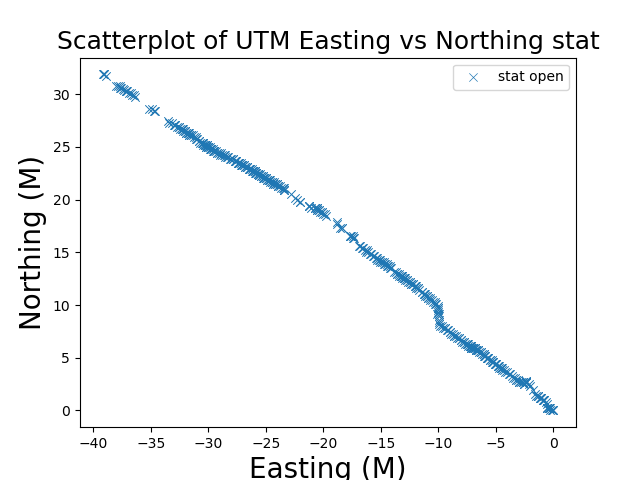
\includegraphics[scale = 0.3]{plot-Scatterplot of UTM Easting vs Northing stat.png}
\end{subfigure}
\begin{subfigure}{}
    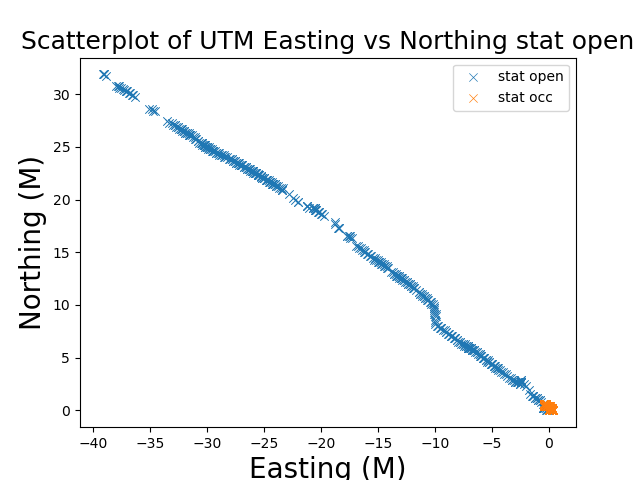
\includegraphics[scale = 0.3]{plot-Scatterplot of UTM Easting vs Northing stat open.png}
\end{subfigure}
\begin{subfigure}{}
    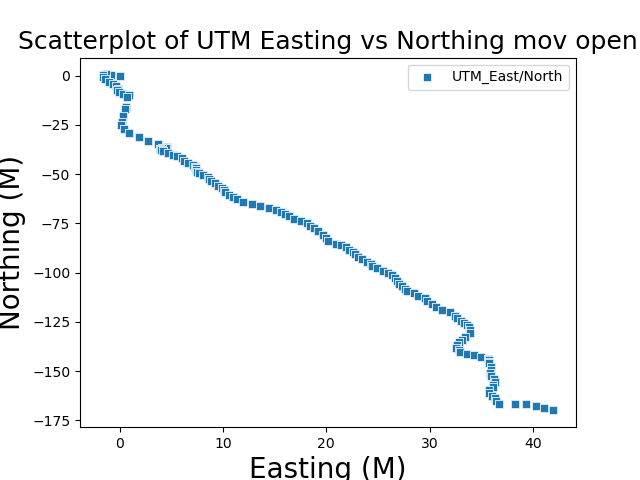
\includegraphics[scale = 0.3]{plot-Scatterplot of UTM Easting vs Northing mov open.png}
\end{subfigure}
\begin{subfigure}{}
    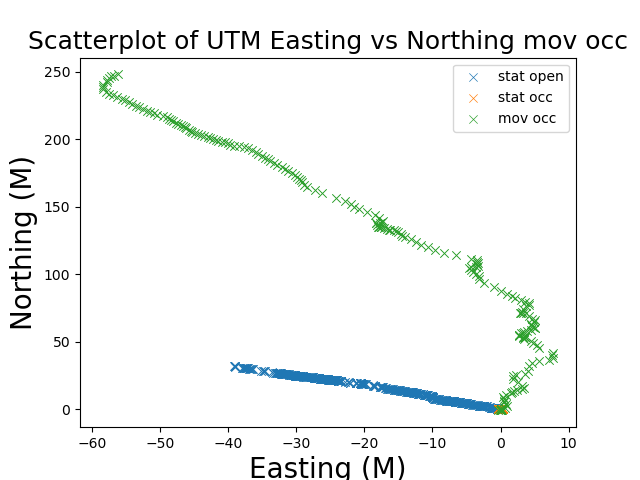
\includegraphics[scale = 0.3]{plot-Scatterplot of UTM Easting vs Northing mov occ.png}
\end{subfigure}
\begin{subfigure}{}
    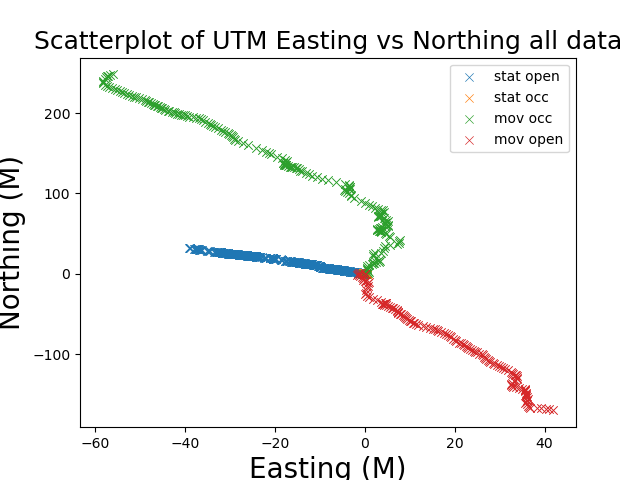
\includegraphics[scale = 0.3]{plot-Scatterplot of UTM Easting vs Northing all data.png}
\end{subfigure}
\caption{UTM Easting vs UTM Northing Scatterplots}
\end{figure}
\subsection{Quantitative error measurement}
Below are the histograms for known position.
\begin{figure}[H]
\begin{subfigure}{}
     \includegraphics[scale = 0.3]{plot-Latitude Histogram for stat occluded.png}
\end{subfigure}
\begin{subfigure}{}
    \includegraphics[scale = 0.3]{plot-Longitude Histogram for stat occluded.png}
\end{subfigure}
\begin{subfigure}{}
    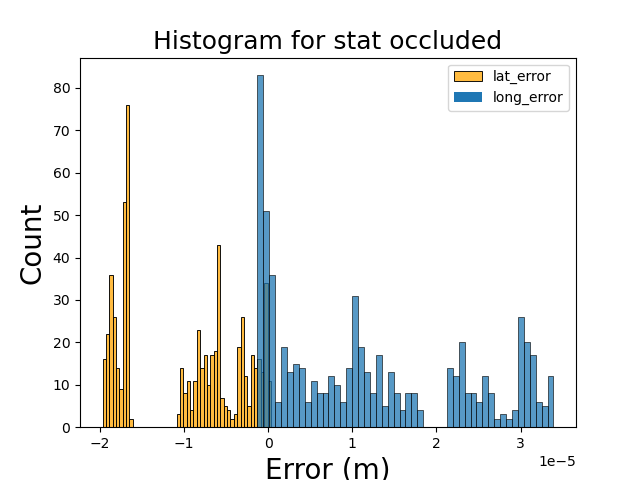
\includegraphics[scale = 0.3]{plot-Histogram for stat occluded.png}
\end{subfigure}
\caption{Histograms of error from known and measured data.}
\end{figure}
\subsubsection{Quantitative error estimation from the known position}
Nowadays we can find more precise and accurate systems and we can use them as our true value. Although we know that getting the exact and precise position on the map is next to impossible, we can consider a similar system as our true value. Hence in this case I used my phone's GPS to get the exact position. For the GPS position in an occluded region, my phone read\\ \\ \textbf{Phone's Lat: 42.3374628, Phone's Long: -71.0900613}.\\ \textbf{Phone's UTM Easting: 327827.25, Phone's UTM Northing: 4689374.84}.\\ \\ 
We cannot directly take the average of the data as averaging considers that the data is uniform and they all have a uniform magnitude of the error. But as we saw from the histograms, it is not the case, the measurement model is \textbf{Nonlinear and Nongaussian model}.\\
One of the most used error analysis methods is to calculate the \textbf{RMSE (Root Mean Square Deviation)} from the actual data and predicted data. Other methods include \textbf{MAPE (Mean Absolute Precision Error)}.
\begin{equation*}
    RMSE=2\sqrt{\frac{1}{N}\sum_{i=1}^N(x_a-x_p)^2}
\end{equation*}
Where $x_a$ is the actual data we got from the GPS puck where as $x_p$ is the predicted value we recorded from the Phone's GPS. To find the singular RMSE value use the below formula. After calculating these data, we got the RMSE values as below...\\
\begin{equation*}
    SRMSE = 2\sqrt{RMSE_{x}^2 + RMSE_{y}^2}
\end{equation*}
Where $RMSE_{x}$ is the RMSE of Latitude or UTM Easting and $RMSE_{y}$ is the RMSE of Longitude or UTM Northing.
\begin{equation*}
    \sigma = 2\sqrt{\frac{1}{N}\sum_{i=1}^N(x_a-\mu)^2}
\end{equation*}
\begin{equation*}
 CEP=0.59(\sigma_e+\sigma_n) =  11.904732100446429
\end{equation*}
$\sigma_e$ = Standard Deviation of UTM Easting and $\sigma_n$ = Standard Deviation of UTM Northing and $\mu$ is the mean of data.
\begin{equation*}
2DRMS=2\sqrt{\sigma_e^2+\sigma_n^2} = 14.330268034155258
\end{equation*}
Note that the above data is in degrees, that is the GPS has an accuracy of 0.001 degrees, we can also convert this data into an approximate meters value by considering the radius of the earth across the equator and poles.\\ \textbf{RMSE value for all data can be found in section 1.5.1}
Furthermore, accurate errors can be calculated by considering the \textbf{CEP (Circular Error Probable)} i.e the percentage of data in CEP with radius X. This can be done by considering the UTM Easting and UTM Northing data and taking its RMSE.
\begin{center}
    \begin{tabularx}{0.8\textwidth} { 
  | >{\centering\arraybackslash}X
  | >{\centering\arraybackslash}X 
  | >{\centering\arraybackslash}X |}
    \hline
    \textbf{Description} & \textbf{Easting (Meters)} & \textbf{Northing (Meters)}\\
    \hline
    \textit{Stationary Occluded} & -40 & 35\\
    \hline
    \textit{Stationary Open} & 0.8 & 0.06\\
    \hline
    \end{tabularx}
\end{center}
\begin{center}
    \begin{tabularx}{0.8\textwidth} { 
    | >{\centering\arraybackslash}X
    | >{\centering\arraybackslash}X |}
    \hline
    \textbf{Singular RMSE in meters for occluded area} & 96.6425\\
    \hline
    \textbf{UTM Easting RMSE} & 72.4973\\
    \hline
    \textbf{UTM Northing RMSE} & 63.9055\\
    \hline
    \end{tabularx}
\end{center}
The above table and scatterplot approximately match hence this RMSE value are significantly correct. Its justification is given below.
\subsubsection{Does this error value make sense given your HDOP value and GPS error in general?}
Although the singular position values and the RMSE were pretty acceptable for all the datasets and given the HDOP value they make sense. But when scatterplots were performed the easting and northing errors in meters do not justify the HDOP value.
In general, the HDOP value is the dilution of precision of the GPS signal and  is a dimensionless quantity. A lower HDOP value suggests better GPS accuracy. While collecting this data I received the HDOp value of around \textbf{0.8 - 0.9} for the occluded region and \textbf{1.0} for the open area. This value cannot be directly compared with the HDOP value due to the quantity\\
\textbf{Note: The justification for the occluded region having more HDOP is probably because the data was collected just beside a metal statue (Sir Shillman's Statue) which caused the signal to be absorbed first by it and then received by a puck. So it kind of amplified the signal, but also amplified the error.}
\subsection{Make a scatterplot of Altitude vs Time}
Below is the scatter plot for altitude vs time for the stationary dataset. It is evident from the graph that the data for an occluded region has more fluctuations and is constantly increasing at a very small rate, whereas the one with an open area has a very small rate of change. \textbf{The below straight line at zero can be neglected as it is by function returning 0 while reading other strings.}
\begin{figure}[H]
\begin{subfigure}{}
     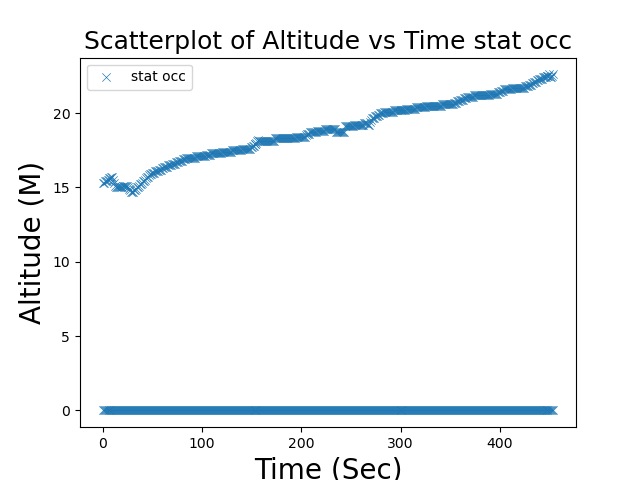
\includegraphics[scale = 0.3]{plot-Scatterplot of Altitude vs Time stat occ.png}
\end{subfigure}
\begin{subfigure}{}
    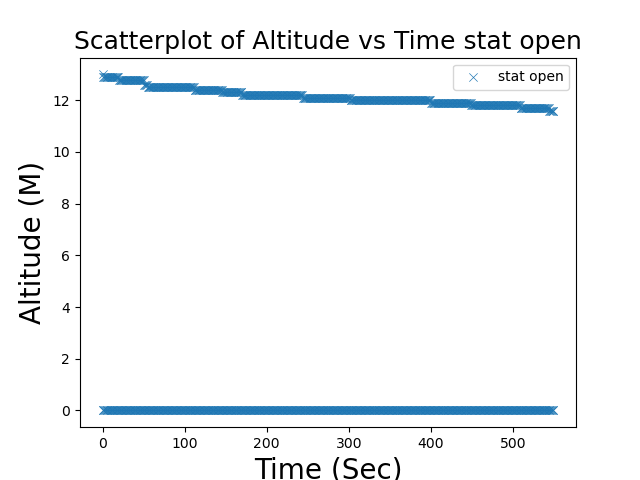
\includegraphics[scale = 0.3]{plot-Scatterplot of Altitude vs Time stat open.png}
\end{subfigure}
\begin{subfigure}{}
    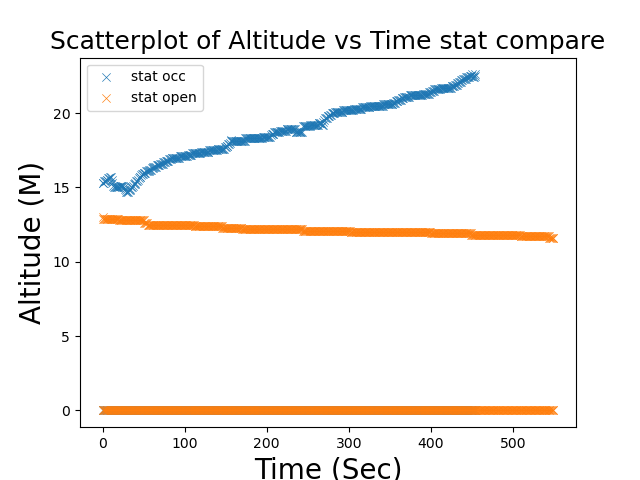
\includegraphics[scale = 0.3]{plot-Scatterplot of Altitude vs Time stat compare.png}
\end{subfigure}
\caption{Altitude vs Time scatterplots}
\end{figure}
\subsection{Analysis on moving data in a straight line}
\subsubsection{Make another scatterplot of northing vs. easting. What’s the error from a line of best fit to your data?}
So far from the above analysis we have seen that one of the best ways of error analysis in such scenarios is calculating the RMSE values. In this case, we have to find the line that best fits the data \textbf{Linear regression or np.polyfit (in python)}. Based on the data calculate the Y-intercept and slope of the line and use that data to find the residuals and find the RMSE value of those data using the equations from the above section. Also, it is evident from the plot that the graph is not linear hence there was so much error due to the \textbf{area surrounded by many tall buildings}. This high error caused the RMSE value to shoot.\\
\textbf{RMSE from a line of best fit to my data was -  24.74569436576671}. Note this value is significantly high as the data we have is in Meters and was collected in a crowded region.\\ Well, the same moving data was collected in an open area with a less occluded region and this time the RMSE value was significant. The below table shows the comparison of errors from data collected in open vs occluded regions with singular RMSE values.\\
\begin{center}
    \begin{tabularx}{0.8\textwidth} { 
  | >{\centering\arraybackslash}X
  | >{\centering\arraybackslash}X |}
 \hline
 \textbf{RMSE for occluded moving data} & 24.74569436576671\\
 \hline
 \textbf{RMSE for open moving data} & 7.886231185022467\\
\hline
\end{tabularx}
\end{center}
\begin{figure}[H]
\begin{subfigure}{}
     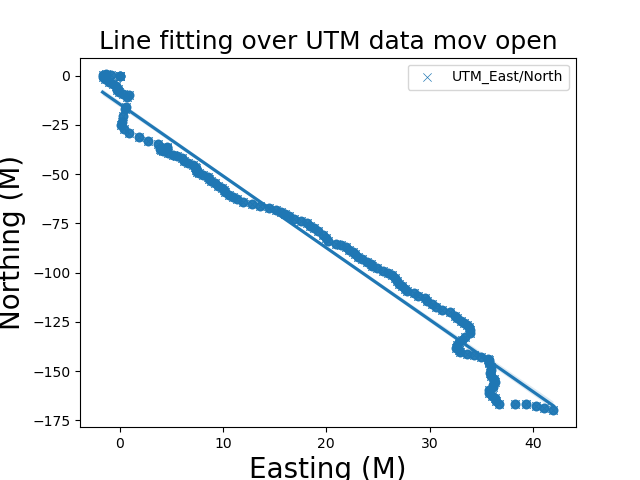
\includegraphics[scale = 0.3]{plot-Line fitting over UTM data mov open.png}
\end{subfigure}
\begin{subfigure}{}
    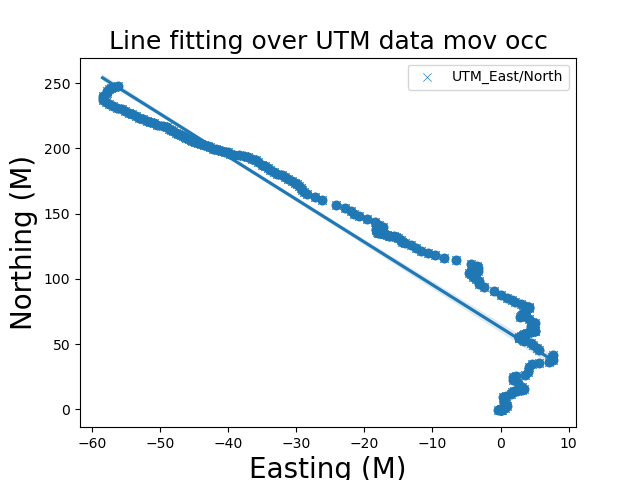
\includegraphics[scale = 0.3]{plot-Line fitting over UTM data mov occ.png}
\end{subfigure}
\begin{subfigure}{}
    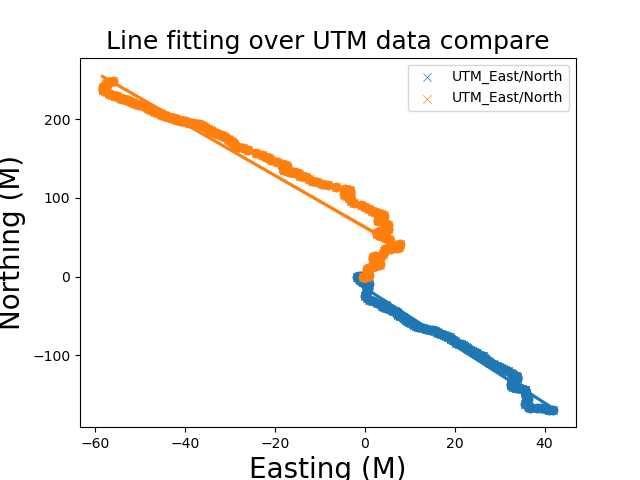
\includegraphics[scale = 0.3]{plot-Line fitting over UTM data compare.png}
\end{subfigure}
\caption{Scatterplots for moving data along with line fitting.}
\end{figure}
\subsubsection{Plot Altitude vs Time Graphs}
Below are the graphs for Altitude vs Time. Note the line at 0 at the bottom of the graph is due to the function returning 0 whenever it reads from a string other than GPGGA as they do not contain the altitude data. We can neglect it in these graphs. The graph for the open region has more errors due to the fact that while collecting the data we constantly had to alter the GPS puck in either hand due to extreme weather.
\begin{figure}[H]
\begin{subfigure}{}
     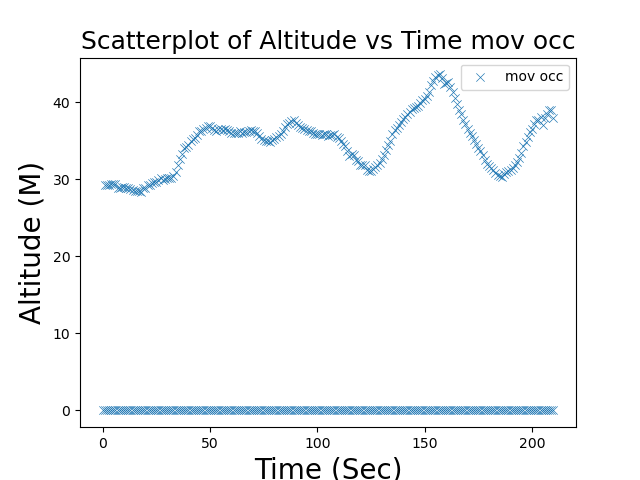
\includegraphics[scale = 0.3]{plot-Scatterplot of Altitude vs Time mov occ.png}
\end{subfigure}
\begin{subfigure}{}
    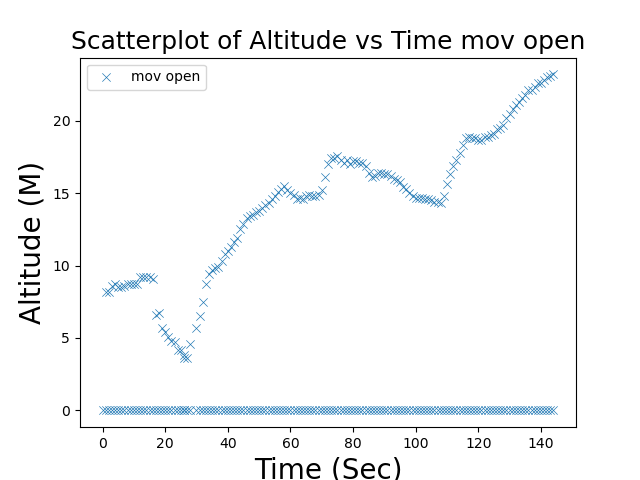
\includegraphics[scale = 0.3]{plot-Scatterplot of Altitude vs Time mov open.png}
\end{subfigure}
\begin{subfigure}{}
    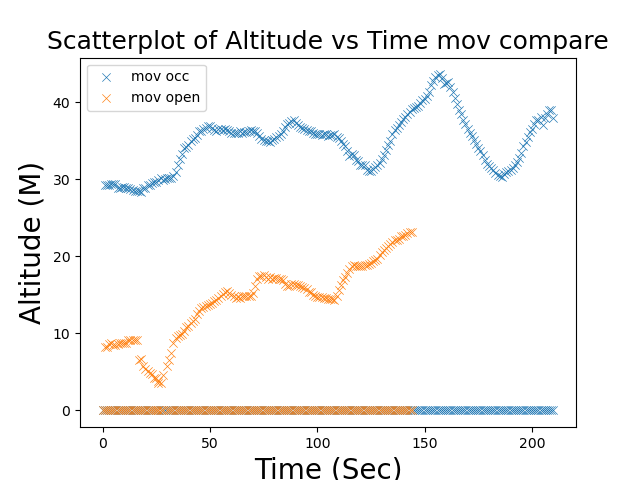
\includegraphics[scale = 0.3]{plot-Scatterplot of Altitude vs Time mov compare.png}
\end{subfigure}
\begin{subfigure}{}
    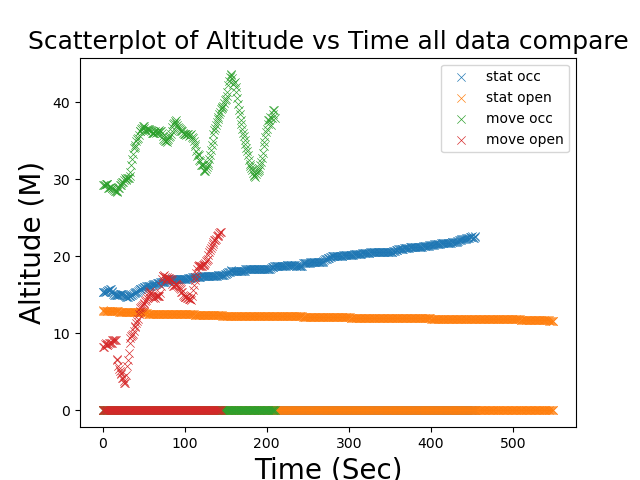
\includegraphics[scale = 0.3]{plot-Scatterplot of Altitude vs Time all data compare.png}
\end{subfigure}
\caption{Scatterplots for Altitude vs Time.}
\end{figure}
\subsection{General Questions}
\subsubsection{How do your estimated error values change for stationary vs. moving data?}
The table below shows a general overview of the error for different data collection. Also do note that these RMSE values are not perfect and precise as there might be errors while converting it from one form to another.\\
\begin{center}
    \begin{tabularx}{0.8\textwidth} { 
  | >{\centering\arraybackslash}X
  | >{\centering\arraybackslash}X 
  | >{\centering\arraybackslash}X |}
    \hline
    \textbf{Description} & \textbf{Open RMSE} & \textbf{Occluded RMSE}\\
    \hline
    \textit{Moving Data} & 7.8862 & 24.7456\\
    \hline
    \textit{Stationary Data} & 0.00105 & 96.6425\\
    \hline
    \end{tabularx}
\end{center}
\subsubsection{GPS navigation while the receiver is moving.}
So far from the above data analysis and the table above we have seen that the RMSE value of the data got significantly higher when our receiver was moving. Hence a brief analysis of this can be that this GPS sensor had errors like \textbf{multipath} which caused the accuracy of GPS data to degrade. Multipath is caused when the GPS signal is reflected by buildings or trees or any other metal and this can cause a significant delay in GPS data received.
\subsubsection{What are physically likely source(s) of error in these data sets?}
As mentioned above the major reason for such significant errors is due to the multipath error due to tall buildings and metal statues in my case proved to be the likely sources of error.
\end{document}
